\documentclass[11pt, headheight=30pt]{scrartcl}
\usepackage[hw]{darkWhite}

\newcolumntype{L}{>{$}l<{$}} % math-mode version of "l" column type
\newcolumntype{C}{>{$}c<{$}} % math-mode version of "c" column type

\DeclareMathOperator{\Mat}{Mat}
\DeclareMathOperator{\diag}{diag}


\title{18.755 Lie Algebra}
\subtitle{Homework 2}
\author{Rowechen Zhong with Isaac Zhu}
\begin{document}

% Exercise 28.3. 1. Let V = C
% n
% , n ≥ 4. Decompose V
% ⊗4 as a direct
% sum of irreducible representations of GLn\text{(sgn+std)} × S4. Characterize the
% occurring Schur functors as spaces of tensors with certain symmetry
% properties, similarly to the above description of S
% (2,1)V . Compute the
% decompositions of V ⊗ S
% 3V , V ⊗ ∧3V , S
% 2V ⊗ S
% 2V, S2V ⊗ ∧2V and
% ∧
% 2V ⊗ ∧2V into Schur functors.
% 2. Decompose V ⊗ V
% ∗
% , V ⊗ V ⊗ V
% ∗
% into a direct sum of irreducible
% representations. Describe the algebra EndGLn\text{(sgn+std)}(V ⊗ V
% ∗ ⊗ V
% ∗
% )
\section{Decomposing $\GL_n(\CC)$-representations}

\begin{prob}
    Let $V = \CC^n, n \geq 4$. Decompose $V^{\otimes 4}$ as a direct sum of irreducible representations of $\GL_n(\CC) \times S_4$. Characterize the occurring Schur functors as spaces of tensors with certain symmetry properties, similarly to the above description of $S^{(2,1)}V$. Compute the decompositions of $V \otimes S^3V, V \otimes \wedge^3V, S^2V \otimes S^2V, S^2V \otimes \wedge ^2V$ and $\wedge ^2V \otimes \wedge ^2V$ into Schur functors.
\end{prob}

The textbook says
\[
    V^{\tensor 3} = \left(S^{(3)}V \tensor \CC_{\text{(tr)}}\right) \oplus \left(S^{(2,1)}V \tensor \CC^2_{\text{(p)}}\right) \oplus \left(S^{(1,1,1)}V \tensor \CC_{\text{(sgn)}}\right).
\]
Tensoring with $V$,
\[
    V^{\tensor 3} \tensor V =  \left(
        S^{(3)}V \tensor \CC_{\text{(tr)}}\right)\tensor V  \oplus \left(S^{(2,1)}V\tensor \CC^2_{\text{(p)}}\right) \tensor V  \oplus \left(S^{(1,1,1)}V \tensor \CC_{\text{(sgn)}}\right)\tensor V 
\]
These are irreps of $S_3$ acting on the first three factors. In addition, we have the decomposition
\begin{align*}
    V^{\tensor 4} &= \left(S^{(4)}V \tensor \CC_{\text{(tr)}}\right) \oplus \left(S^{(3,1)}V \tensor \CC^3_{\text{(std)}}\right) \oplus \left(S^{(2,2)}V \tensor \CC^2_{}\right)\\
    &\oplus \left(S^{(2,1,1)}V \tensor \CC^3_{\text{(sgn+std)}}\right) \oplus \left(S^{(1,1,1,1)}V \tensor \CC_{\text{(sgn)}}\right)
\end{align*}
where $\CC_{\text{(tr)}}, \CC^3_{\text{(std)}}, \CC^2_{}, \CC^3_{\text{(sgn+std)}}, \CC_{\text{(sgn)}}$ are the irreps of $S_4$, as described by the character table:
\begin{center}
\begin{tabular}{c|ccccc}
    $S_4$ & $e$ & $(12)$ & $(123)$ & $(12)(34)$ & $(1234)$ \\
    \hline
    $\CC_{\text{(tr)}}$ & 1 & 1 & 1 & 1 & 1 \\
    $\CC^3_{\text{(std)}}$ & 3 & 1 & 0 & -1 & -1 \\
    $\CC^2_{}$ & 2 & 0 & -1 & 2 & 0 \\
    $\CC^3_{\text{(sgn+std)}}$ & 3 & -1 & 0 & -1 & 1 \\
    $\CC_{\text{(sgn)}}$ & 1 & -1 & 1 & 1 & -1 
\end{tabular}
\end{center}

The way you compute this is sort of involved, as far as I can tell.
\begin{itemize}
    \item We know that $S^{(4)}$ pairs with $\CC_{tr}$ and $S^{(1,1,1,1)}$ pairs with $\CC_{sgn}$.
    \item We wish to determine $\Hom_{\GL_n(\CC)}(S^{(3,1)}V, V^{\otimes 4})$. Our strategy is to track the highest weight vectors as representatives. These must live in the $4$-dimensional subspace spanned by $e_1\otimes e_1\otimes e_1\otimes e_2$ by cyclic permutations. In order to be a highest weight vector, it needs to be annihilated by raising $e_2\to e_1$, so it is the subspace where these $4$ coefficients sum to $0$; this is the \vocab{standard representation}. You can tell that this is $\CC^3_{\text{(std)}}$ and not $\CC^3_{}$ because $(1234)$ acts by $-1$ on this subspace.
    \item We wish to determine $\Hom_{\GL_n(\CC)}(S^{(2,2)}V, V^{\otimes 4})$. The highest weight vectors embed into the $6$-dimensional subspace spanned by $e_1\otimes e_1\otimes e_2\otimes e_2$ by cyclic permutations. In order to be a highest weight vector, it needs to be annihilated by raising $e_2\to e_1$. It is quickly checked that this is the case iff the coefficient on $e_1\otimes e_1\otimes e_2\otimes e_2$ is equal to that of $e_2\otimes e_2\otimes e_1\otimes e_1$ (and cyclically equivalent conditions), plus the sum of all coefficients is $0$. This yields a $2$-dimensional space, which must be $\CC^2_{}$.
    \item Finally, the remaining representation must be $\CC^3_{\text{(sgn+std)}}$.
\end{itemize}

When we restrict to $S_3\to S_4\to \End V^{\tensor 4}$ acting on the first three factors of $V^{\tensor 4}$, each of the $S_4$-irreps split into $S_3$-irreps as
\begin{align*}
    \CC_{\text{(tr)}} &\to \CC_{\text{(tr)}} \\
    \CC^3_{\text{(std)}} &\to \CC_{\text{(tr)}} \oplus \CC^2_{\text{(p)}} \\
    \CC^2_{} &\to \CC^2_{\text{(p)}} \\
    \CC^3_{\text{(sgn+std)}} &\to \CC_{\text{(sgn)}} \oplus \CC^2_{\text{(p)}} \\
    \CC_{\text{(sgn)}} &\to \CC_{\text{(sgn)}}
\end{align*}
Matching up $S_3$ irreps, we have
\begin{align*}
    S^{(3)}V \tensor V &= S^{(4)}V \oplus S^{(3,1)}V \\
    S^{(2,1)}V \tensor V &= S^{(3,1)}V \oplus S^{(2,2)}V \oplus S^{(2,1,1)}V \\
    S^{(1,1,1)}V \tensor V &= S^{(2,1,1)}V \oplus S^{(1,1,1,1)}V
\end{align*}
So we can characterize:
\begin{itemize}
    \item $S^{(3,1)}V$ is the space of tensors symmetric in the first three components, with full symmetrization zero
    \item $S^{(2,1,1)}V$ is the space of tensors antisymmetric in the first three components, with full antisymmetrization zero
\end{itemize}

Observe
\begin{align*}
    V^{\tensor 2} &= \left(S^{(2)}V \tensor \CC_{\text{(tr)}}\right) \oplus \left(S^{(1,1)}V \tensor \CC_{\text{(sgn)}}\right)
\end{align*}
The irreps of $S_2 \times S_2$ are:
\begin{center}
\begin{tabular}{c|cccc}
    $S_2 \times S_2$ & $e$ & $(12)$ & $(34)$ & $(12)(34)$ \\
    \hline
    $\chi_{\text{(tr)}} \equiv \CC_{\text{(tr)}} \tensor \CC_{\text{(tr)}}$ & 1 & 1 & 1 & 1 \\
    $\chi_1 \equiv \CC_{\text{(tr)}} \tensor \CC_{\text{(sgn)}}$ & 1 & 1 & -1 & -1\\
    $\chi_2 \equiv \CC_{\text{(sgn)}} \tensor \CC_{\text{(tr)}}$ & 1 & -1 & 1 & -1\\
    $\chi_3 \equiv \CC_{\text{(sgn)}} \tensor \CC_{\text{(sgn)}}$ & 1 & -1 & -1 & 1
\end{tabular}
\end{center}

We can decompose $V^{\tensor 2} \tensor V^{\tensor 2}$ into irreps of $S_2 \times S_2$:
\begin{align*}
    V^{\tensor 2} \tensor V^{\tensor 2} &= \left(S^{(2)}V \tensor S^{(2)}V \tensor \chi_{\text{(tr)}}\right) \oplus \left(S^{(2)}V \tensor S^{(1,1)}V \tensor \chi_1 \right) \\
    &\oplus \left(S^{(1,1)}V \tensor S^{(2)}V \tensor \chi_2 \right) \oplus \left(S^{(1,1)}V \tensor S^{(1,1)}V \tensor \chi_{3}\right).
\end{align*}

We can compare this against the Schur-Weyl decomposition of $V^{\tensor 4}$. The $S_4$-irreps split as
\begin{align*}
    \CC_{\text{(tr)}} &\to \chi_{\text{(tr)}} \\
    \CC^3_{\text{(std)}} &\to \chi_{\text{(tr)}} \oplus \chi_1 \oplus \chi_2 \\
    \CC^2_{} &\to \chi_{\text{(tr)}} \oplus \chi_3 \\
    \CC^3_{\text{(sgn+std)}} &\to \chi_1 \oplus \chi_2 \oplus \chi_3 \\
    \CC_{\text{(sgn)}} &\to \chi_3
\end{align*}
Matching up $S_2 \times S_2$-irreps gives 
\begin{align*}
    S^{(2)}V \tensor S^{(2)}V &= S^{(4)}V \oplus S^{(3,1)}V \oplus S^{(2,2)}V \\
    S^{(2)}V \tensor S^{(1,1)}V &= S^{(3,1)}V \oplus S^{(2,1,1)}V \\
    S^{(1,1)}V \tensor S^{(1,1)}V &= S^{(2,2)}V \oplus S^{(2,1,1)}V \oplus S^{(1,1,1,1)}V
\end{align*}
Thus, $S^{(2,2)}V$ is the space of tensors symmetric in the first two components and symmetric in the last two components, with vanishing symmetrization in the first three components.

\begin{prob}
    Decompose $V \otimes V^*, V \otimes V \otimes V^*$ into a direct sum of irreducible representations. Describe the algebra $\End_{\GL_n(\CC)}(V \otimes V^* \otimes V^*)$.
\end{prob}

Over $\sl_n$, $\rho = \frac12(n-1, n-3, \dots, -n+1)$ is the half-sum of positive roots. In the Weyl character formula we will be using always contract this against a zero-sum element, so we will write $\rho = (n,\dots, 1)$.

$V\otimes V^*$ is a very special case. The $n$ weights of $V$ are all permutations of $(1,0,\dots, 0)$, and the $n$ weights of $V^*$ are all permutations of $(1,\dots,1,0)$, thus the $n^2$ weights of $V$ contain all $n^2 - n$ permutations of $(2,1,\dots,1,0)$ with multiplicity $1$ and $(1,\dots,1)$ with multiplicity $n$. The highest weight is $(2,1,\dots,1,0)$. The finite-dimensional representation with highest weight $(2,1,\dots,1,0)$ is actually just the adjoint representation of $\sl_n$ on itself, which notably has dimension $n^2 - 1$. Thus the weight space of the adjoint representation contains all $n^2 - n$ permutations of $(2,1,\dots, 1,0)$ with multiplicity $1$, and a weight space $(1,\dots,1)$ with multiplicity $n-1$. The remaining weight $(1,\dots, 1)$ lies in the one-dimensional determinant representation. Thus, we find
\[
    V\otimes V^* = \ad \oplus \det = L_{(2,1,\dots,1,0)} \oplus L_{(1,\dots,1)}  
\]

Meanwhile, $V\otimes V\otimes V^*$ will be much more complex. Here is a table with all of the information:
\begin{center}
\begin{tabular}{C|C|C|C|C|C}
    \text{Dominant Weight} & \text{Permutations} & V\otimes V \otimes V^* & L_{(3,1,\dots,1,0)} & L_{(2,2,1,\dots,1,0)} & L_{(2,1,\dots,1)}\\
    (3,1,\dots,1,0) & n(n-1) & 1 & 1 & 0 & 0 \\
    (2,2,1,\dots,1,0) & \frac{n(n-1)(n-2)}{2} & 2 & 1 & 1 & 0 \\
    (2,1,\dots,1) & n & 2n-1 & n-1 & n-2  & 1\\
    \hline
    \text{Total Dimension} & & n^3 & \frac{(n+2)n(n-1)}{2} & \frac{(n+1)n(n-2)}{2} & n
\end{tabular}
\end{center}

The first column shows each dominant weight with nonzero multiplicity inside $V\otimes V\otimes V^*$. The second column shows the cardinality of the image of these elements under the Weyl group. The following columns show the dimensions of the corresponding weight spaces, and the total dimension of the representations. The column of $V\otimes V\otimes V^*$ is computed easily; the operation of tensoring two representations simply tensors each of their weight spaces, so it amounts to computing a convolution; it's just combinatorics.

The total dimensions in the last row are computed from the Weyl dimension formula;
\[
    \dim L_\lambda = \frac{\prod_{\alpha\in\Phi^+} \langle \lambda + \rho, \alpha\rangle}{\prod_{\alpha\in\Phi^+} \langle \rho, \alpha\rangle}    
\]
This is easier than it seems, because $O(n^2)$ of the terms are the same, leaving only $O(n)$ terms to compute. Let's work out $(3,1,\dots,1,0)$.
\[
    \lambda + \rho = (n + 3, n, n - 1,\dots, 3, 1)
\]
Any $\alpha \in \Phi^*$ takes the form $\alpha = e_i - e_j$ and $i < j$. If $i \neq 1$ and $j \neq n$, then $\braket{\lambda + \rho, \alpha} = \braket{\rho, \alpha}$. Thus, we need only consider the following terms:
\begin{itemize}
    \item When $\alpha = e_1 - e_j$, with $1 < j < n$, the quotient is $\frac{j + 1}{j-1}$. This product telescopes to $\frac{n(n-1)}{2}$.
    \item When $\alpha = e_i - e_n$, with $1 < i < n$, the quotient is $\frac{n-i +1}{n-i}$. This product telescopes to $n-1$.
    \item Finally, if $\alpha = e_1 - e_n$, the quotient is $\frac{n+2}{n-1}$.
\end{itemize}
The full dimension is thus $\frac{(n+2)n(n-1)}{2}$, as claimed.

Now let's work out$(2,2,1,\dots,1,0)$.
\[
    \lambda + \rho = (n + 2, n + 1, n - 1,\dots, 3, 1)
\]
Any $\alpha \in \Phi^*$ takes the form $\alpha = e_i - e_j$ and $i < j$. If $i \notin \{1,2\}$ and $j \neq n$, then $\braket{\lambda + \rho, \alpha} = \braket{\rho, \alpha}$. Thus, we need only consider the following terms:
\begin{itemize}
    \item When $\alpha = e_1 - e_j$, with $2 < j < n$, the quotient is $\frac{j}{j-1}$. This product telescopes to $\frac{n-1}{2}$.
    \item When $\alpha = e_2 - e_j$, with $2 < j < n$, the quotient is $\frac{j-1}{j-2}$. This product telescopes to $n-2$.
    \item When $\alpha = e_i - e_n$, with $2 < i < n$, the quotient is $\frac{n-i +1}{n-i}$. This product telescopes to $n-2$.
    \item Finally, if $\alpha = e_1 - e_n$, the quotient is $\frac{n+1}{n-1}$, if $\alpha = e_2 - e_n$, the quotient is $\frac{n}{n-2}$, and if $\alpha = e_1 - e_2$, the quotient is $1$.
\end{itemize}
The full dimension is thus $\frac{(n+1)n(n-2)}{2}$, as claimed.

The final computation required is the dimension of $\mu = (2,2,1,\dots,1,0)$ inside $L_\lambda$ with $\lambda = (3,1,\dots,1,0)$. For this, we use the Kostant multiplicity formula, which states that
\[
    \dim L_\mu = \sum_{w\in W} (-1)^w p(w(\lambda + \rho) - (\mu + \rho)).
\]
This turns out to be trivial, because while $W = S_n$, it is clear that any permutation $w\neq 1$ of $\lambda + \rho$ will cause $w(\lambda + \rho) \prec \mu + \rho$. Of course $p(\lambda - \mu) = 1$.

The penultimate row containing the dimensions of $(2,1,\dots,1)$ can be computed by subtracting out the total dimension.

Anyways, if you look at the table, it is completely clear that
\[
    V\otimes V\otimes V^* = L_{(3,1,\dots,1,0)} \oplus L_{(2,2,1,\dots,1,0)} \oplus L^{\otimes 2}_{(2,1,\dots,1)}.   
\]
By symmetry,
\[
    V\otimes V^* \otimes V^* = L_{(3,2,\dots,2,0)} \oplus L_{(2,1,\dots,1,0,0)} \oplus L^{\otimes 2}_{(1,\dots,1,0)}.    
\]

By Schur's theorem, $\End_{GL_n(\CC)}(V \otimes V^* \otimes V^*) = \Mat_1(\CC) \oplus \Mat_1(\CC) \oplus \Mat_2(\CC) \cong \CC^6$; we simply map between the multiplicity spaces.


\section{Decomposing $\SL_3(\CC)$ weight spaces}

\setcounter{prob*}{1}
\begin{prob*}
    Draw the weights of the representation $S^{(2,2)}\CC^3$ of $\SL_3(\CC)$ on the hexagonal lattice, and indicate their multiplicities.
\end{prob*}

The highest weight of $S^{(2,2)}$ is $(\lambda_1, \lambda_2, \lambda_3) = (2,2,0) = 2\omega_2$, the rightmost red dot. The orange arrows in the diagram below are the basis of the roots, and the red dots are the weights. The red arrows represent applying the lowering operators.

Each of the six weight spaces has multiplicity 1.

\begin{center}
    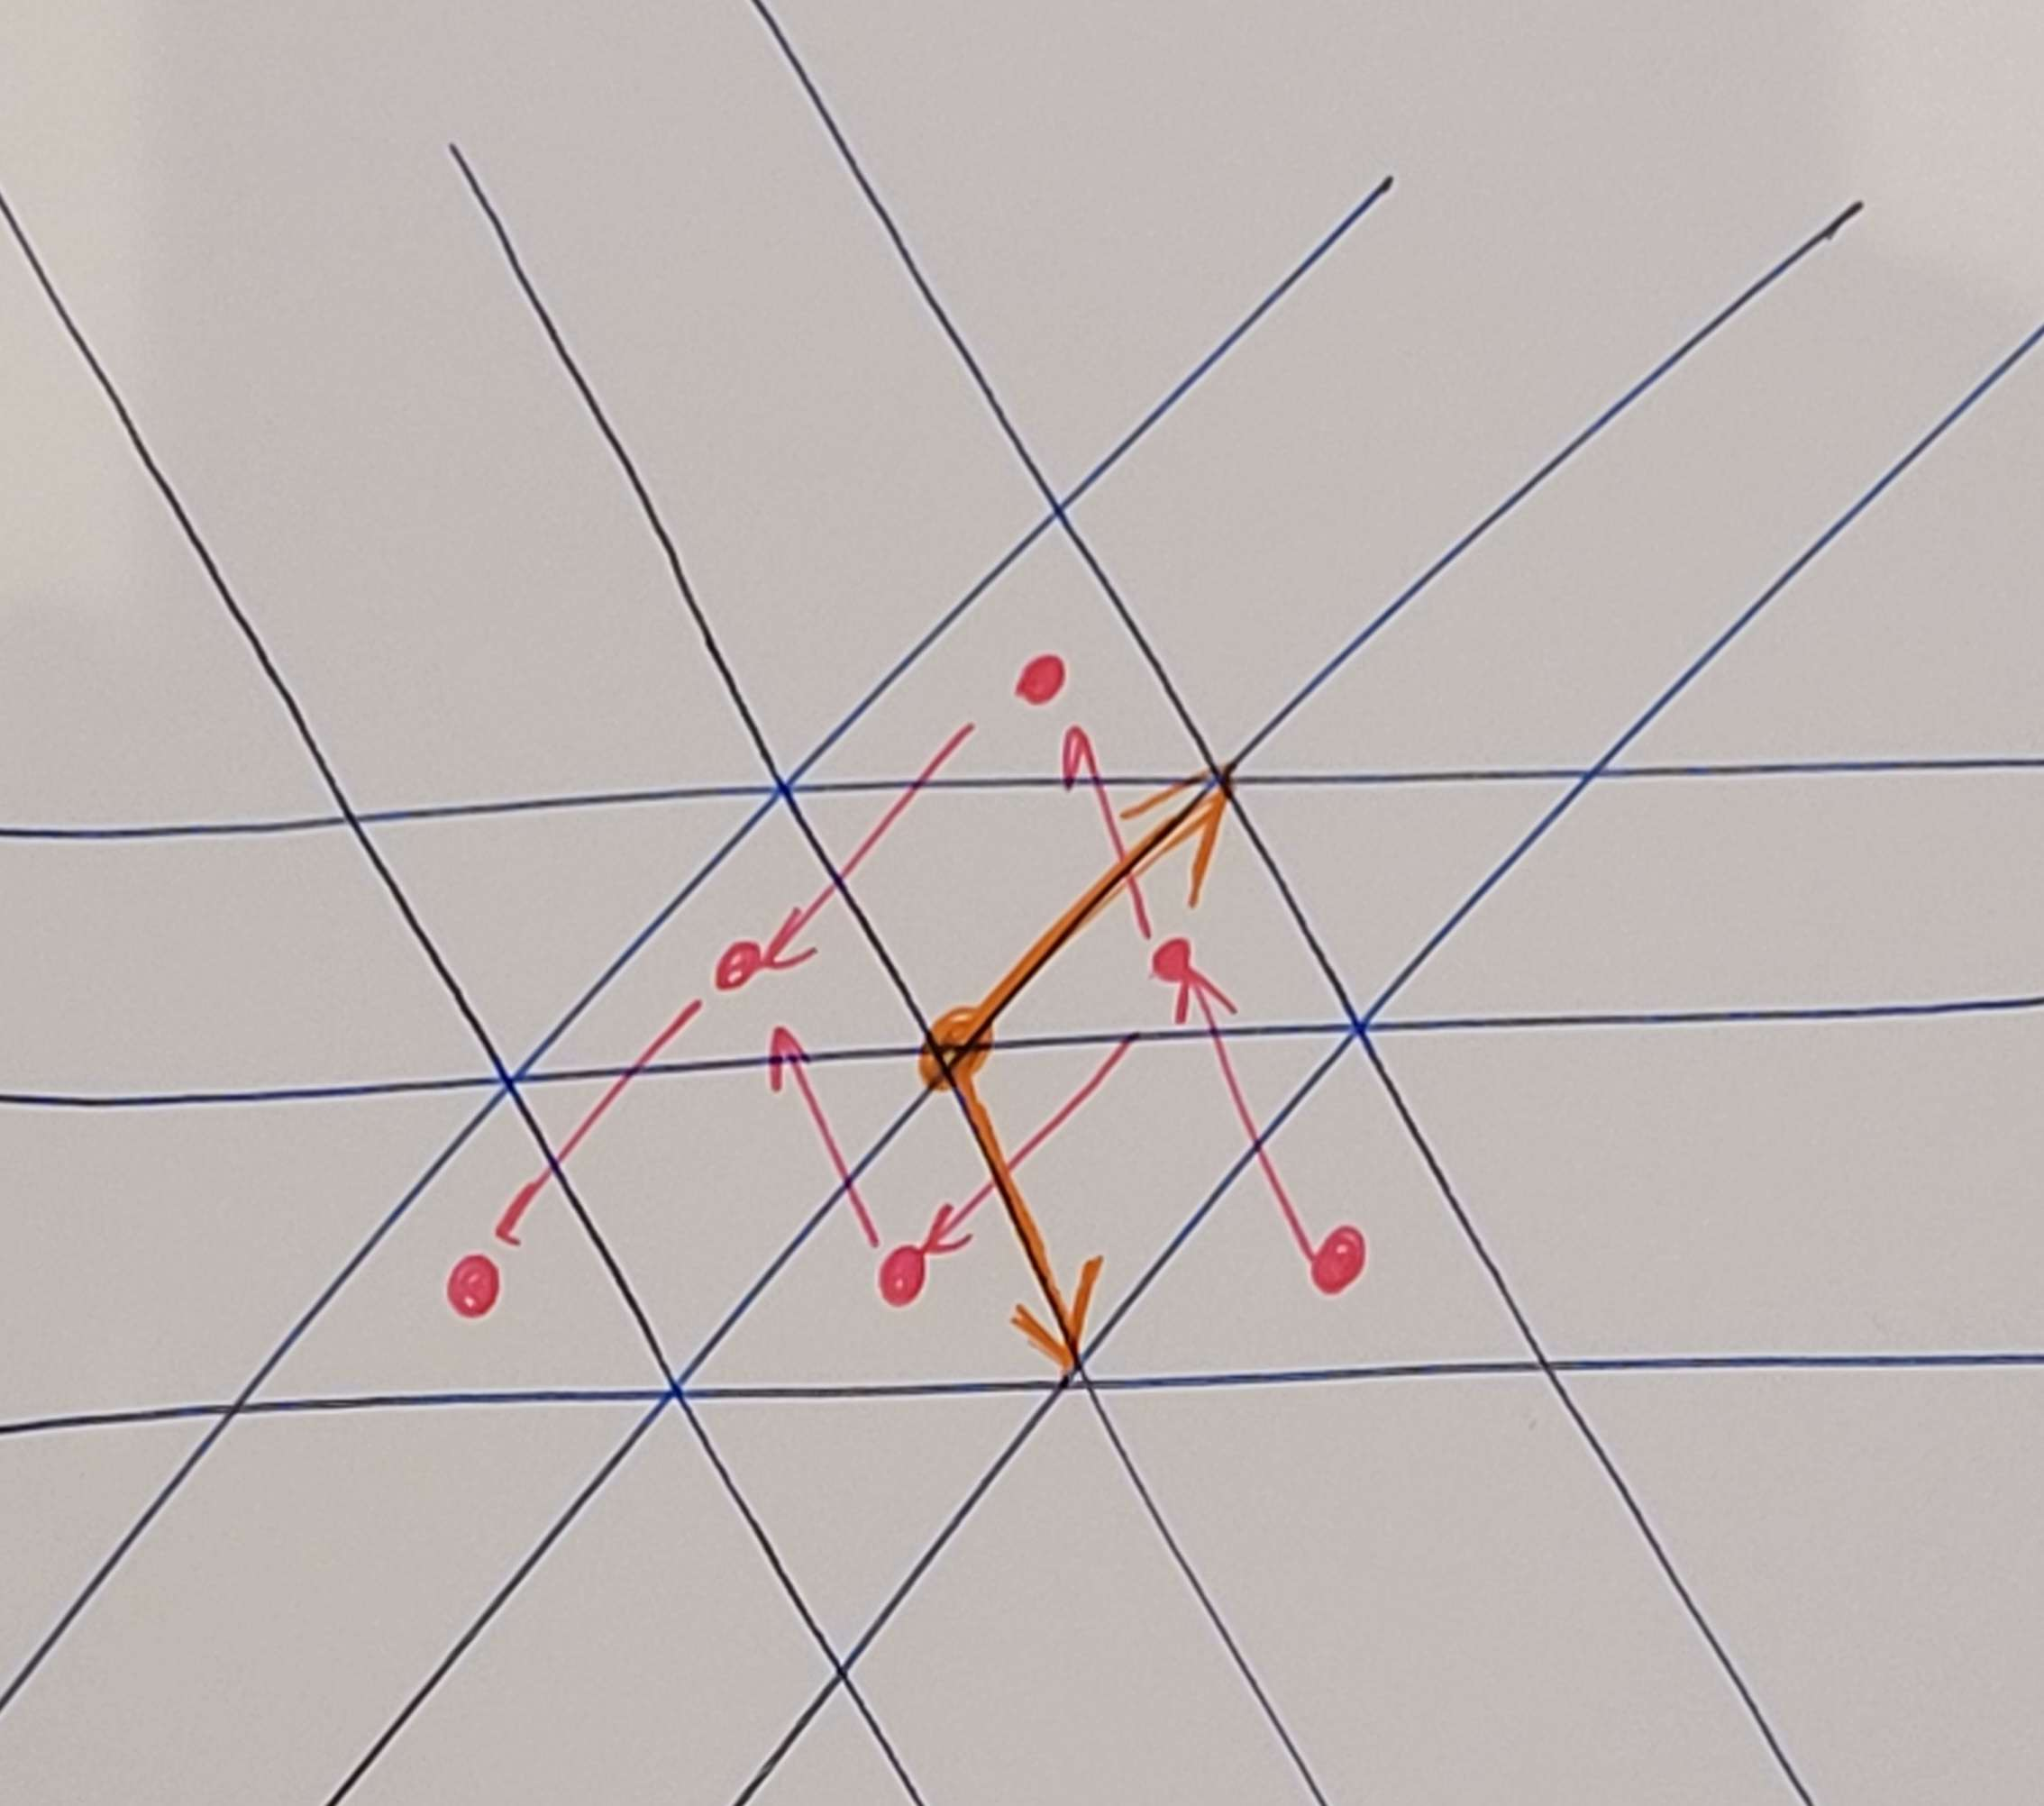
\includegraphics[width=0.5\textwidth]{SL3_weight.jpg}
\end{center}


\section{Amitsur-Levitzki identity}

\setcounter{prob*}{2}
\begin{prob*}
    Let $X_1, \dots, X_{2n}$ be complex $n \times n$ matrices. Let $\Lambda = \wedge(\xi_1, \dots, \xi_{2n})$ be the exterior algebra generated by $\xi_i$ with relations $\xi_i \xi_j = -\xi_j \xi_i, \xi_i^2 = 0$. Let $X$ be the matrix over $\Lambda$ given by $X := X_1 \xi_1 + \cdots + X_{2n} \xi_{2n}$.
\end{prob*}
\begin{prob}
    Let $Y = X^2$. Show that $Y \in \Mat_n(\Lambda^+)$ where $\Lambda^+$ is the commutative subalgebra of $\Lambda$ spanned by the elements of even degrees. Compute $Y^n$.
\end{prob}
$Y = X^2 = \sum_{i,j} X_i X_j \xi_i \xi_j$. Each $\xi_i \xi_j$ has even degree, so $Y$ is a matrix over the commutative subalgebra $\Lambda^+$. $Y^n = X^{2n}$ has degree $2n$, so it can be written as some matrix multiple of $\xi_1 \dots \xi_{2n}$ by anticommuting the $\xi$'s;
\begin{align*}
    Y^n &= X^{2n}\\
        &= \sum_{\sigma \in S_{2n}} X_{\sigma(1)} \cdots X_{\sigma(2n)} \xi_{\sigma(1)} \cdots \xi_{\sigma(2n)}\\
        &= \sum_{\sigma \in S_{2n}} \sgn(\sigma) X_{\sigma(1)} \cdots X_{\sigma(2n)} \xi_1 \cdots \xi_{2n}
\end{align*}

\begin{prob}
    Show that $\Tr(Y^k) = 0 \in \Lambda^+$ for $k = 1, \dots, n$.
\end{prob}
\[
    Y^k = X^{2k} = \sum X_{i_1} \cdots X_{i_{2k}} \xi_{i_1} \cdots \xi_{i_{2k}}
\]
Where the sum is over tuples $(i_1, \dots, i_{2k})$ of distinct indices. Any fixed $\{i_1, \dots, i_{2k}\}$ contributes the following to the above sum:
\[
    \sum_{\sigma \in S_{2k}} \sgn(\sigma) X_{i_{\sigma(1)}} \cdots X_{i_{\sigma(2k)}} \xi_{i_{\sigma(1)}} \cdots \xi_{i_{\sigma(2k)}} = \xi_1 \cdots \xi_{2k} \sum_{\sigma \in S_{2k}} \sgn(\sigma) X_{i_{\sigma(1)}} \cdots X_{i_{\sigma(2k)}} 
\]
The RHS pairs up as
\[X_{i_{\sigma(1)}} X_{i_{\sigma(2)}} \cdots X_{i_{\sigma(2k)}} - X_{i_{\sigma(2)}} \cdots X_{i_{\sigma(2k)}} X_{i_{\sigma(1)}}\]
which are traceless by the cyclic property of trace. Thus $Y^k$ is traceless for $k = 1, \dots, n$.

\begin{prob}
    Deduce that $Y^n = 0$. This should yield the Amitsur-Levitzki identity
    \[
    \sum_{\sigma \in S_{2n}} \sgn(\sigma) X_{\sigma(1)} \dots X_{\sigma(2n)} = 0.
    \]
\end{prob}
We rephrase this purely algebraically. For any matrix $Y \in \mathrm{Mat}_n(A)$ for a commutative algebra $A$, if we have $\Tr(Y^k) = 0$ for $k = 1, \dots, n$, then $Y^n = 0$.

In the case where $A = \CC$, we can diagonalize, so this is easy. The eigenvalues $\lambda_1, \dots, \lambda_n$ of $Y$ satisfy $\lambda_1^k + \cdots + \lambda_n^k = 0$ for $k = 1, \dots, n$, which implies the characteristic polynomial of $Y$ is $t^n$. Thus $Y$ is nilpotent. $Y$ is $n \times n$, thus $Y^n = 0$.

However, this means that if we consider $Y$ as an element of $\CC^{n^2}$, then the $n$ polynomial equations given by $\Tr(Y^k)=0$ algebraically imply that $Y^n$ vanishes! This algebraic relation must extend to any commutative ring $A$.

Thus, the expression found from part 1 yields
\[
    \sum_{\sigma \in S_{2n}} \sgn(\sigma) X_{\sigma(1)} \dots X_{\sigma(2n)} = 0.
\]

\begin{prob}
    Deduce the same identity over any commutative ring $R$.
\end{prob}

The Amitsur-Levitzki identity is a polynomial identity in the matrices $X_1, \dots, X_{2n}$; it is a purely algebraic fact. This immediately generalizes to any commutative ring $R$.


\section{Decomposing $V^{\otimes N}$}
\setcounter{prob*}{3}

\begin{prob*}
    Let $V = \CC^2$ be the 2-dimensional tautological representation of $\GL_2(\CC)$. Decompose $V^{\otimes N}$ into a direct sum of irreducible representations of $\GL_2(\CC) \times S_N$ and compute the characters and dimensions of all the irreducible representations of $\GL_2$ and $S_N$ that occur.
\end{prob*}

The Schur-Weyl decomposition reads
\[
    V^{\otimes N} = \bigoplus_{|\lambda|=N} L_\lambda \otimes \pi_\lambda
\]
where $\lambda = (a+b,b)$ for nonnegative integers $a,b$ with $a+2b=N$.

By the Weyl character formula (see page 138 calculation), the character of $L_\lambda$ is
\[
    \chi_\lambda(\diag(x,y)) = \frac{x^{a+b+1}y^{b} - x^{b}y^{a+b+1}}{x-y} = (xy)^{b} \frac{x^{a+1}-y^{a+1}}{x-y}
\]
To find the dimension of $L_\lambda$, we plug in $x=y=1$ which (under the obvious limit) yields $\dim L_\lambda = a+1$.

We now consider $\pi_\lambda$ as an irrep of $\CC[S_N]$. The Frobenius formula says $\chi_\lambda(\sigma)$ is the coefficient of $x^{a+b+1} y^b$ in the polynomial
\[
    (x-y) \prod_{i=1}^N (x^i + y^i)^{m_i}
\]
where $m_i$ is the number of cycles of length $i$ in $\sigma$. Finally, to find the dimension of $\pi_\lambda$, plug in $\sigma = 1$, such that all cycles have length $1$:
\[
    \dim \pi_\lambda = \binom{N}{b} - \binom{N}{b-1} = \frac{N-2b+1}{N+1} \binom{N+1}{b}
\]
\end{document}